\section{讨论:连接数可扩放性}
\label{socksdirect:sec:discussion}


使用商用 RDMA 网卡时,\sys {} 对大量连接的可伸缩性受共享内存和RDMA的限制。
为了表明 \libipc {} 和监视器不是瓶颈,本节在两个重用RDMA QP和共享内存的进程之间创建了很多连接。使用 \libipc {} 的应用程序线程每秒可以创建1.4~M个新连接,这是Linux的20倍和mTCP的2倍 \cite {jeong2014mtcp}。监视器每秒可以创建5.3~M个连接。

由于主机内的进程数量有限,因此SHM连接的数量可能不会很大。
但是,一台主机可能连接到许多其他主机,RDMA的可扩展性成为一个问题。
RDMA 的可扩展性归结为两个问题。
首先,RDMA 网卡使用网卡内存作为缓存来保持每个连接状态。当有数千个并发连接时,性能受到频繁缓存未命中的影响 \cite {mprdma,kaminsky2016design,kalia2018datacenter}。
因为 RDMA 传统上部署在中小型集群中,传统 RDMA 网卡上的内存容量较小。
随着近年来大规模的 RDMA 部署 \cite {guo2016rdma},商用网卡拥有更大的内存来存储数千个连接 \cite {kalia2018datacenter},而本文使用的可编程网卡拥有数千兆字节的DRAM~ \cite {mellanox-innova,mellanox-bluefield,smartnic}。
因此,本文预测未来的数据中心不会为网卡缓存未命中问题担心过多。下一节将基于可编程网卡,提出一个连接数可扩放的传输层实现框架。
第二个问题是本文的测试平台中建立RDMA连接需要大约 $30 \mu s$,这对于短连接很重要。此过程仅涉及本地CPU和网卡之间的通信,因此这个连接建立延迟是可以优化的。

除了大量并发连接,服务质量保证(Quality of Service,QoS)也是数据中心的重要需求。
传统网络协议栈在操作系统内核实现服务质量保证。
而对于本章使用的硬件传输协议,将数据平面性能隔离和拥塞控制卸载到 RDMA 网卡上是一个越来越流行的研究方向 \cite {peter2016arrakis,zhu2015congestion,lu2017memory,mprdma,mittal2018revisiting},因为数据中心的网卡正变得越来越可编程  \cite{smartnic,cavium,kaufmann2015flexnic,mellanox-innova,mellanox-bluefield},而且公有云已经在虚拟机之外的网络功能中提供了 QoS \cite {li2016clicknp,panda2016netbricks,floem-osdi18}。

连接数可扩放性需要存储每个连接的传输层和数据包缓冲区。针对传输层状态问题,接下来的两节提出两种方案:在可编程网卡中或主机 CPU 的用户态库中存储连接状态并实现传输层处理。针对数据包缓冲区问题,最后一节提出多套接字共享队列,将两个进程间多个连接的缓冲区合并。

\subsection{基于可编程网卡的传输层}
\label{socksdirect:sec:smartnic}

%\textbf{Communicating with TCP/IP peers.}
%We use a user-space networking stack to communicate with regular TCP/IP peers, but the compatibility may be limited~\cite{yasukata2016stackmap}.
%To solve this problem, after receiving the TCP SYN+ACK, the monitor can create an established kernel TCP connection using TCP connection repair~\cite{tcp-connection-repair}.
%Moreover, if the application and monitor share a network namespace, the monitor can send the kernel 文件描述符 to the application via Unix domain socket, then \libipc{} can use the 文件描述符 without delegation to the monitor.

%\textbf{Connecting to many RDMA capable hosts.}
%With a lot of hosts, the 网卡 still suffer from performance degradation due to large number of connections.
%In contrast, user-space networking stack alleviates this problem because the 网卡 is stateless.
%We provide a socket option to enable applications to delegate operations to the monitor and use user-space networking stack even if the peer supports RDMA.
%An application can choose to use RDMA for latency sensitive and throughput demanding connections, and user-space networking stack for others.






本节基于可编程网卡和第 \ref{chapter:socksdirect} 章的网络数据包处理平台和第 \ref{chapter:kvdirect} 章的内存键值存储,实现了一个连接数可扩放的 RDMA 网卡。
实现连接数可扩放的主要挑战是在缓存不命中率很高时,高吞吐量地存取主机内存中的连接状态,并能隐藏存取延迟。这正是第 \ref{chapter:kvdirect} 章所解决的问题,因此本节基于高性能键值存储实现了可扩放的连接状态存储。


\begin{figure}[htbp]
	\centering
	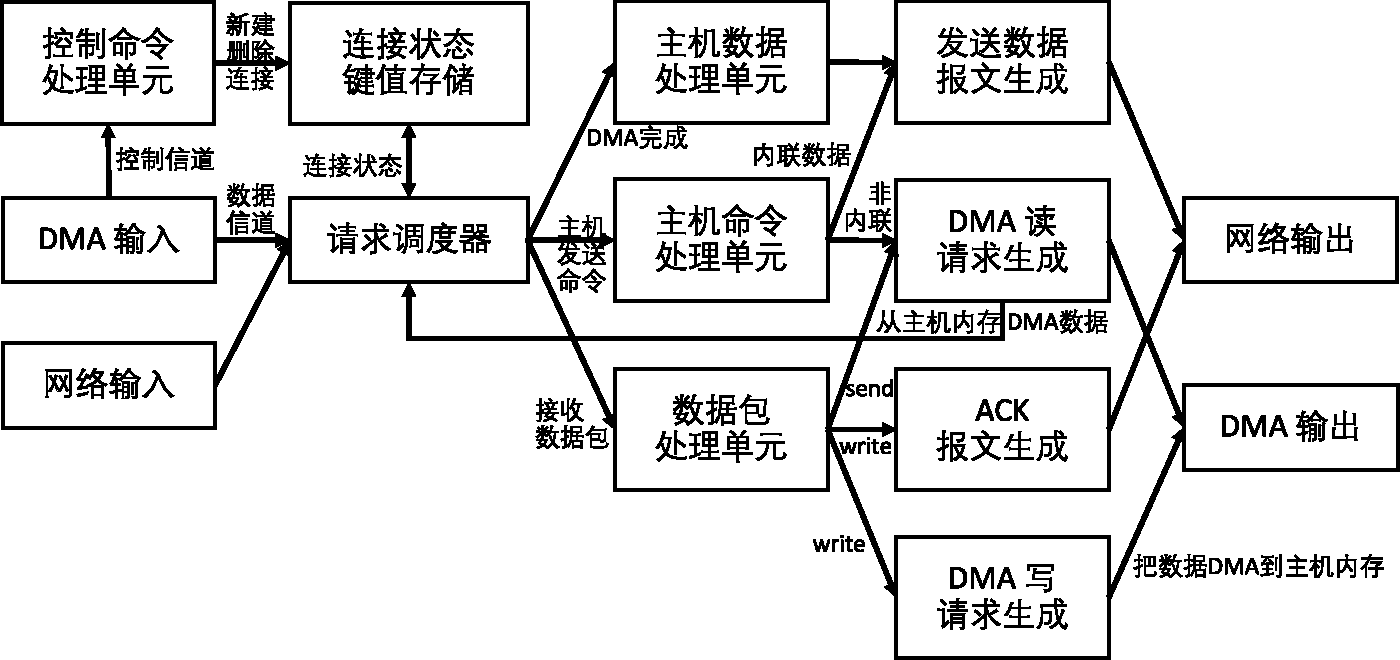
\includegraphics[width=1.0\textwidth]{images/scalable_rdma.pdf}	
	\caption{基于可编程网卡的连接数可扩放 RDMA。}
	\label{socksdirect:fig:scalable-rdma}
\end{figure}

基于可编程网卡的 RDMA 网卡架构如图 \ref{socksdirect:fig:scalable-rdma} 所示。
RDMA 网卡需要处理来自主机的控制和数据传输命令(工作请求,work request),还需要处理来自网络的数据包。
对于控制和数据传输命令,主机 CPU 把工作请求放入主机内存中的工作队列(work queue),再通过 PCIe DMA 发送到网卡 \cite{kalia2016design}。
通过网络接口接收的数据包也被放入网卡的输入缓冲区,对应工作队列中的一个工作请求。
请求调度器根据数据包的五元组(five-tuple)信息或主机命令中的连接编号,从连接状态键值存储中取出连接的状态信息,并按照连接的优先级,将工作请求和当前连接状态分类放入网卡内部的不同工作队列。
由于 RDMA 消息的处理是有状态的,处理同一个连接的两个相邻数据包可能存在依赖关系。为此,请求调度器记录正在处理的连接,并只调度未被处理连接的工作请求,这与第 \ref{chapter:kvdirect} 章键值存储中同一个键的消息处理方式相同。
对于接收到的数据包,接收处理单元按照 RDMA 消息的类型处理。对于 RDMA 单边写(write)消息,只需生成主机 DMA 操作,将数据写入主机内存的相应位置,并回复 ACK 消息。对于 RDMA 单边读(read)、原子(atomic)和双边发送(send)消息,需要从主机内存中读取相应的数据,才能进行下一步操作。为了隐藏主机内存读取的 DMA 延迟,生成主机内存的 DMA 读请求后,还需要生成一个新的工作请求,等待 DMA 完成后再进行下一步处理。
这种新工作请求被送回请求调度器,同时标记等待条件。
当 DMA 完成后,请求调度器将处理这个新工作请求,发送数据到网络或将数据 DMA 到主机内存。
数据发送命令 send 的处理方式与 RDMA 单边读(read)消息的处理方式类似。
数据接收命令 recv 不需要网卡主动处理,而是从网络收到双边发送(send)或带立即数的单边写(write with immediate)消息时,才需要匹配对应的 recv 工作请求。

上述处理流程的性能挑战是单个时钟周期内很难完成一个工作请求的有状态处理(如拥塞控制),而同一个连接的工作请求不能并行处理,从而降低了单连接吞吐量。解决方案是将工作请求的处理流水线(pipeline)化,每个流水级(stage)处理连接状态的不同部分,因此流水级之间没有数据依赖。在每个流水级内设置第 \ref{chapter:kvdirect} 章的数据转发(data forwarding)机制,使尚未写回请求调度器的状态更新对后续的工作请求可见。这样,同一个连接有依赖关系的多个工作请求可以在不同的流水级间并发处理。对于这类可以通过流水线和数据转发解决的依赖,请求调度器就不必记录依赖关系,而是认为所有此类请求都是不相关的。


\subsection{基于 CPU 的传输层}

实现连接数可扩放性的另一种方案是在主机 CPU 上实现传输层协议,从而网卡无需为每个连接存储状态,只需实现无状态卸载。
用户态协议栈与网卡之间使用收发数据包接口,而非 RDMA 消息接口。
我们利用 DPDK 等高性能数据包处理框架实现主机 CPU 与网卡间的高效通信。
基于 LibVMA 实现……





\subsection{多套接字共享队列}
\label{socksdirect:subsec:multiplex-conn}

很多应用在两个进程间建立多个套接字连接。




%\textbf{Multiplex connections in event-driven applications.}
To reduce memory footprint and improve locality of memory accesses, we use one queue to multiplex all connections between a pair of threads. Each data item in the queue is marked with its 文件描述符. By using a single queue, we reduce per-socket memory footprint, random memory accesses and cache misses.

\textbf{Message format.}
As shown in Figure~\ref{socksdirect:fig:locklessq-structure}, the main component of the queue is a \emph{data ring buffer}, where messages are stored back-to-back.
Each message in the ring buffer consists of an 8-byte header and a variably sized payload. The header consists of an \textit{isvalid} flag, an opcode, the receiver's 文件描述符 number and the payload size. Messages are aligned to 8 bytes to ensure header write atomicity.% and accelerate payload copy.



\begin{figure}[htbp]
	\centering
	\subfloat[传统队列结构。]{
		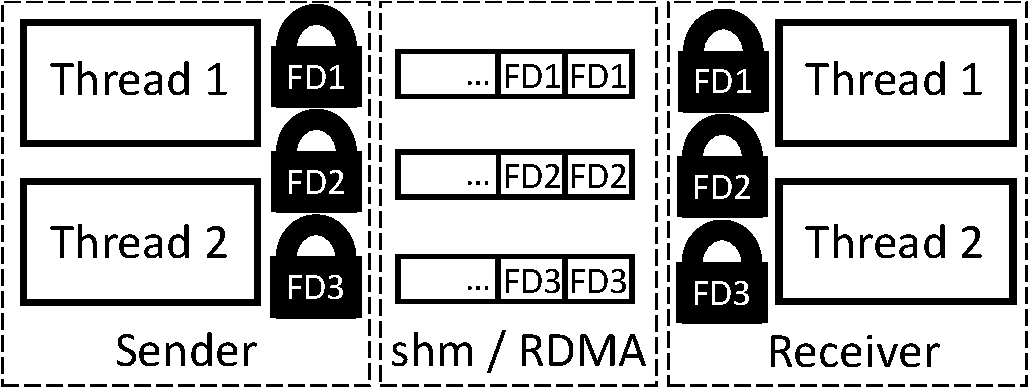
\includegraphics[width=0.6\textwidth]{images/fork_linux}
	}

	\subfloat[多套接字共享队列结构。]{
		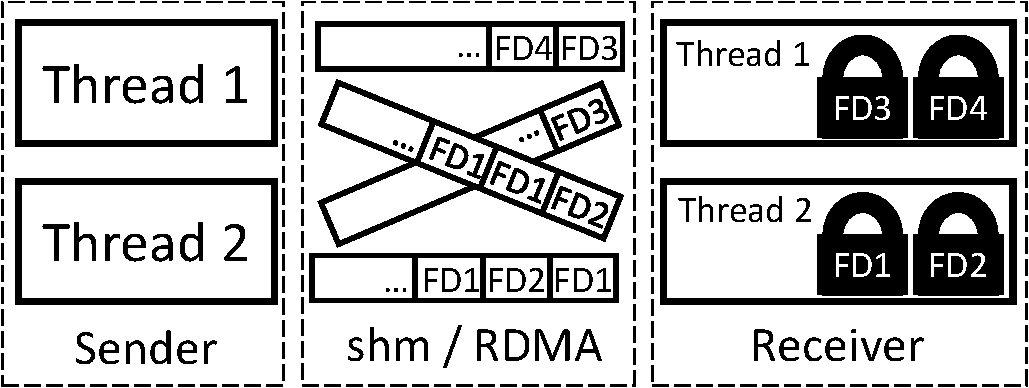
\includegraphics[width=0.6\textwidth]{images/fork_rdwr}
	}
	\caption{队列结构的比较。 假设发送者和接收者各有两个线程。 首先,\ sys {}在每对发送方和接收方线程之间创建对等队列。 我们不是用锁来保护队列,而是将每个文件描述符指定给接收者线程以确保排序。 其次,来自所有连接(文件描述符)的数据通过共享队列进行多路复用,而不是每个文件描述符一个队列。}
	\label{socksdirect:fig:fork-rdwr}
\end{figure}

\iffalse
\begin{figure}[htbp]
	\centering
	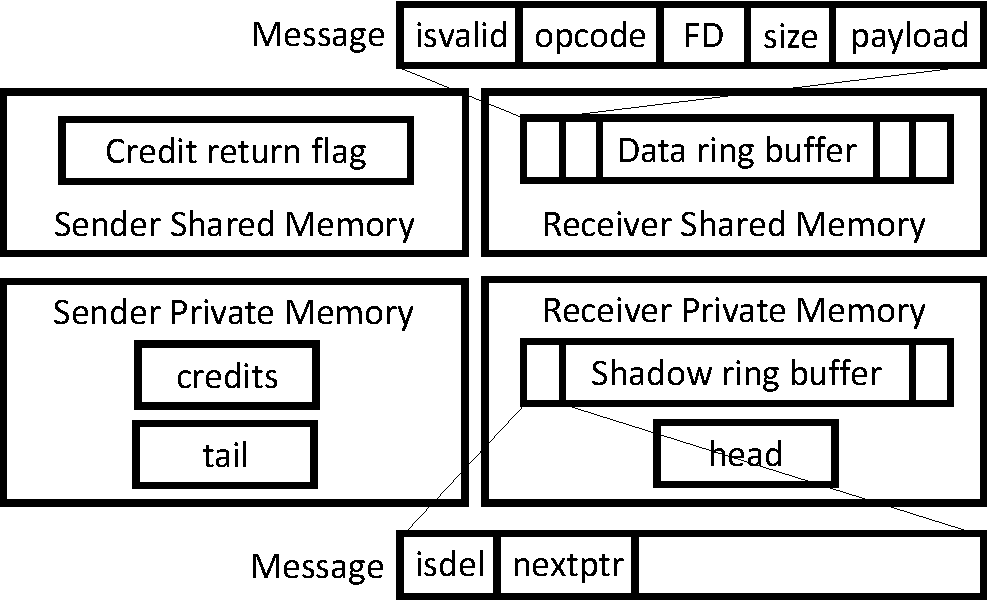
\includegraphics[width=0.8\textwidth]{images/locklessq_new}
	
	\caption{The structure of an inter-process queue.}
	
	\label{socksdirect:fig:locklessq-structure}
\end{figure}
\fi

\textbf{Event polling.}
We maintain a bitmap of each epoll 文件描述符 set.
When \texttt{epoll\_wait} is called, we scan all data queues round-robin and check the 文件描述符 of each data message against the bitmap. If the 文件描述符 is in the bitmap, an event is returned to the application.
A global cursor exists to resume data queue scanning from the last position in the last scanned queue.

A per-queue cursor records the last scanned position in each queue to avoid scanning a message multiple times.
To speedup repeated receive operations of a specific 文件描述符, we build a linked list of messages for each 文件描述符 as a side product of event polling.
Each 文件描述符 maintains positions of the first and last scanned but unread messages of the 文件描述符.
When a new message of the 文件描述符 is scanned, the \emph{nextptr} pointer in the last message is updated to point to the new message.

To poll events from sockets and other 文件描述符 (handled by kernel) at the same time, \libipc{} creates an \textit{epoll thread} in each process to wait on all 文件描述符 handled by kernel. When it receives a kernel event, it broadcasts the event to application threads via shared memory queues. %\texttt{Epoll\_wait} in \libipc{} will return such kernel events in addition to socket events. %Note that Linux allows an event to be received by multiple threads sharing the 文件描述符.

\textbf{Pick from middle of queue.}
In order to support receiving data from a specific 文件描述符, the queue needs to support picking a message in the middle with a specific 文件描述符.
Fortunately, this does not happen frequently. Event-driven applications typically process incoming events in a FIFO order. For \texttt{epoll\_wait} in level trigger mode, we iterate through all messages in the queue and return those in the set of registered 文件描述符. When applications call \texttt{recv}, \libipc{} would usually dequeue the message at head.

To pick from middle of queue, receiver traverses messages in the ring buffer. During traversal, receiver iterates messages from \textit{head} until free space in ring buffer, determined by \textit{isvalid}. Hence, receiver cannot clear \textit{isvalid} when a non-head message is dequeued. That's why each message has an \textit{isdel} flag. When a message is dequeued from the middle, its \textit{isdel} is set. %If the message at \textit{head} has \textit{isdel} set, the receiver advances \textit{head} and repeats this step.

\textbf{Head-of-line blocking.}
%Second, if application does not receive from a 文件描述符 for a long time, data items of the 文件描述符 may fill up the queue and starve other 文件描述符.
If application does not receive from a 文件描述符 for a long time, the empty space in queue will become fragmented.
When data queue is full, the sender sends a message via emergency queue to trigger garbage collection in the receiver.
The receiver scans empty space in the middle of queue and moves remaining messages, so that empty space can be returned to the sender.
%To avoid starvation, we need at least one byte of headroom per 文件描述符. Accordingly, we design a single byte \textit{headroom slot} per 文件描述符. When data queue is full and the per-文件描述符 headroom slot is free, sender uses it and sends a notification via emergency queue. Receiver receives from data queue first, then from the headroom slot if it received a notification.

\textbf{Emergency queue.}
Control messages may need to be delivered out-of-band when the queue is full. For example, in order to close the receive direction while sending data, the shutdown message should not be blocked by unconsumed data in the queue. To this end, we add an \textit{emergency queue} alongside each data queue.
A receiver will always retrieve messages in the emergency queue immediately.


%\subsubsection{Zero Copy TCP}
%\label{socksdirect:subsec:zero-copy-tcp}
%
%For TCP connections, we optimize the user-space TCP/IP stack to remove memory copy between \libipc{} and 网卡.
%Because the payloads of sent and received packets need to align at 4~KiB page boundary, we leverage scatter-gather support in modern 网卡s~\cite{mellanox} to separate packet header from application payload.
%%During initialization, \libipc{} queries IP and Ethernet MAC address from the kernel and constructs a packet header template.
%For \texttt{send}, \libipc{} constructs a packet header to a 网卡 send work request, then fills in the payload buffer address from application. 
%For receiving data, in background, \libipc{} issues 网卡 receive work requests with a 54-byte buffer to store Ethernet, IPv4 and TCP headers, followed by a page-aligned buffer to store payload.
%%In corner cases where the received header length is not 54 bytes, \libipc{} reassembles the packet.
%Upon \texttt{recv}, the payload buffer is remapped to application.



图 \ref{socksdirect:fig:eval-connnum-tput} 显示了不同并发连接数量下的单核吞吐量。
测试前在两个主机间预先建立指定数量的连接,然后轮流(round-robin)使用这些连接以乒乓(ping-pong)的模式收发数据。
\sys{} 可以用 4 GB 的可编程网卡 DRAM 内存支持 100 M 条并发连接,并且在如此高的并发度下吞吐量不降低。
作为对比,RDMA、LibVMA 和 Linux 的性能随连接数量的增加而迅速降低。
对于 RDMA,性能在超过 512 条并发连接后迅速降低,这是由于 RDMA 传输层状态占满了网卡缓冲区。
尽管 LibVMA 和 Linux 并不使用 RDMA 作为传输层,它们为每条连接维护缓冲区,因此在数千条并发连接时会导致 CPU 缓存和 TLB 不命中。
此外,LibVMA 在网卡中为每个连接安装了一条连接重定向规则(flow steering rule),这也会导致网卡缓存不命中。

\begin{figure}[htbp]
	\centering
	\subfloat[单机内吞吐量。]{                    
		%\begin{minipage}{0.4\textwidth}
		\centering
		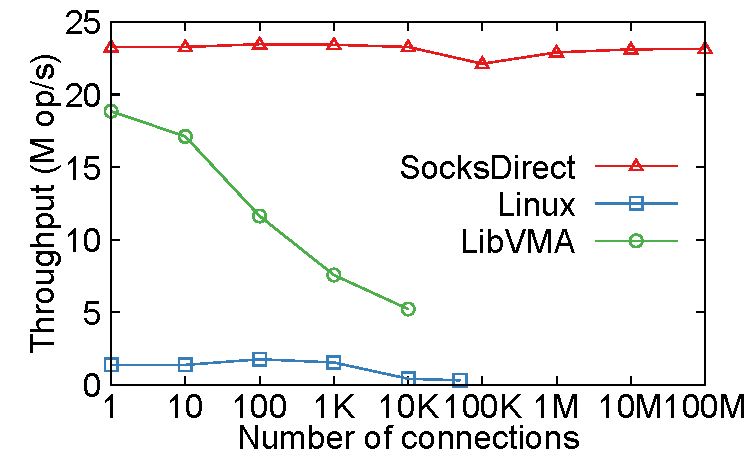
\includegraphics[width=0.5\textwidth]{eval/microbenchmark/connnum-ipc-tput.pdf}
		\label{socksdirect:fig:eval-connnum-ipc-tput}
		%\end{minipage}
	}
	\subfloat[跨主机吞吐量。]{
		%\begin{minipage}{0.4\textwidth}
		\centering 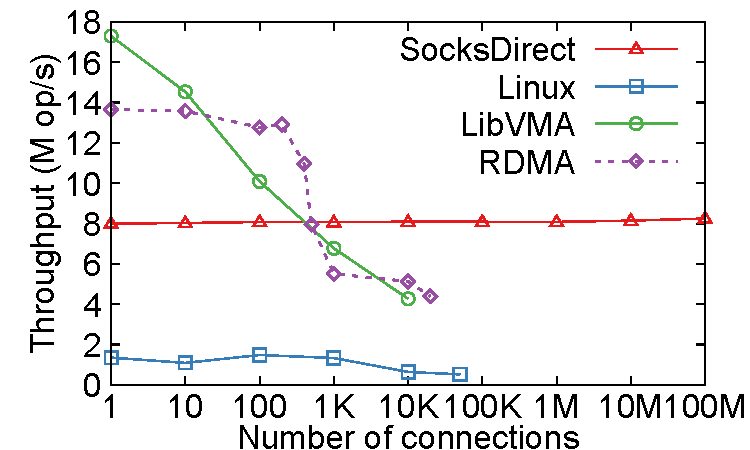
\includegraphics[width=0.5\textwidth]{eval/microbenchmark/connnum-network-tput.pdf}
		\label{socksdirect:fig:eval-connnum-network-tput}
		%\end{minipage}
	}
	
	\caption{不同并发连接数量下的单核吞吐量。}
	\label{socksdirect:fig:eval-connnum-tput}
\end{figure}




\section{讨论:应用、协议栈与网卡间的接口抽象}
\label{socksdirect:sec:api-discussion}

应用程序与用户态协议栈之间使用套接字接口。协议栈与网卡间使用 RDMA 接口。任务划分?不仅是性能问题,接口容易编程?






%Another promising direction to solve the RDMA concurrency issue is to implement the reliable transport in CPU, and the 网卡 remains stateless. However, RDMA UD does not support one-sided write, so the ring buffer in Sec.~\ref{socksdirect:subsec:lockless-queue} will not work. Existing software RDMA~\cite{soft-roce} has low performance. It would be interesting to co-design software and 网卡.

%\textbf{Networking stack on other layers.}
%RDMA: lower layer,
%eRPC, message queue, etc: higher layer.

%\section{Related Work}
%\label{socksdirect:sec:related-work}

%Several mostly related works have been discussed in Sec.~\ref{socksdirect:subsec:related-work}.

\iffalse
\parab{Linux kernel optimization.}
One line of research optimizes the kernel stack for higher socket performance. FastSocket~\cite{lin2016scalable} and Affinity-Accept~\cite{pesterev2012improving} scale connection creation to multiple cores, but synchronization is still needed when multiple threads share a socket.
FlexSC~\cite{soares2010flexsc} proposes exception-less system calls to reduce kernel crossing overhead.
Zero-copy socket~\cite{thadani1995efficient,chu1996zero} still needs copy-on-write on senders.
In addition, they fail to remove cache miss and transport overheads.


\parab{New OS stacks.}
Another line of research proposes new OS stacks with modified socket interface, mostly aiming at zero copy and fast event notification. Existing socket applications need modifications to use the new interfaces.
For intra-server connections, Arrakis~\cite{peter2016arrakis} and IX~\cite{belay2017ix} use the 网卡 to forward packets from one process to another. The hairpin latency from CPU to 网卡 is at least two PCIe delays, which is one order of magnitude higher than inter-core cache migration delay. In addition, the data plane switching throughput of a 网卡 is constrained by PCIe bandwidth (Figure~\ref{socksdirect:fig:eval-corenum-tput}).

For inter-server connections, most OS stacks implement transport in software. IX~\cite{belay2017ix} and Stackmap~\cite{yasukata2016stackmap} run in the kernel to enforce QoS policy or preserve protocol compatibility with Linux, while Arrakis~\cite{peter2016arrakis} and SandStorm~\cite{marinos2014network} run in user mode to maximize performance.
RDMA and transport virtualization~\cite{tsai2017lite,niu2017network} also enforce QoS in the hypervisor.
Due to the additional level of indirection, kernel stacks cannot remove kernel crossing, while batched syscalls add latency.
Further, large-scale deployment of kernel-based stacks is more complicated than user-space libraries~\cite{andromeda}.
\sys offloads transport and QoS to 网卡 hardware.
RDMA transport has been deployed in many data centers~\cite{guo2016rdma}, and an emerging line of work~\cite{zhu2015congestion,lu2017memory,mprdma} improves congestion control and QoS in large-scale RDMA deployments.
For flexibility, programmable 网卡s are being adopted in data centers~\cite{smartnic,cavium}, as they are more efficient than general-purpose CPUs for network processing~\cite{kaufmann2015flexnic,li2016clicknp}.



\parab{User-space socket.}
A third line of research runs socket in user space.
mTCP~\cite{jeong2014mtcp}, Seastar~\cite{seastar}, 
F-stack~\cite{fstack} and LOS~\cite{huang2017high} use a high performance packet I/O framework (\textit{e.g.} netmap~\cite{rizzo2012netmap}, DPDK~\cite{dpdk} and PF\_RING~\cite{pf-ring}) and achieves compatibility with most Linux socket functions and scalability with number of cores and sockets.
LibVMA~\cite{libvma}, OpenOnload~\cite{openonload} and DBL~\cite{dbl} are fully compatible with existing applications. However, they use vendor-specific 网卡 features and do not scale to multiple threads or connections.
In addition, user-space sockets do not support zero copy or efficient multitasking.

Most user-space sockets focus on inter-server and do not optimize for intra-server connections.
FreeFlow~\cite{freeflow} uses shared memory for intra-server communication and RDMA for inter-server, but it provides an RDMA interface.
Existing socket to RDMA translation approaches, \textit{e.g.} SDP~\cite{socketsdirect} and rsockets~\cite{rsockets} are not fully compatible with Linux and do not address scalability challenges.


%\parab{RDMA.}
%First, RDMA is not suitable for WAN. Second, RDMA has scalability issue when one server connects to many servers. Software transport in CPU access connection states in host memory, while hardware RDMA transport caches connection states in 网卡 and swaps out to host memory when cache overflows. First, CPU cache miss costs less than 0.1$\mu$s, while 网卡 cache miss costs 0.5$\mu$s~\cite{kaminsky2016design}. Second, CPU memory bandwidth is an order of magnitude larger than 网卡 PCIe bandwidth. In light of this, a host should switch to software transport when it actively communicates with a large number of hosts. Fortunately, Modern 网卡s has an increasing size of memory and supports more active connections without performance degradation~\cite{kaminsky2016design}.
\fi


\iffalse
\begin{itemize}
	\item New abstraction (RDMA, lwip + DPDK etc.) 
	\begin{itemize}
		\item 
	\end{itemize}
	\item Compatible with socket (libvma, LOS etc.) 
	\begin{itemize}
		\item Violate goal 2: memory copy 
		\item Violate goal 3: thread synchronization for multi-thread applications 
	\end{itemize}
	\item Common problems: 
	\begin{itemize}
		\item Designed for networking, does not support or optimize for IPC communication inside the same server 
		\item Violate goal 4: Not optimized for many connections 
	\end{itemize}
\end{itemize}
\fi

